%!TEX root = ../Diploma.tex

\clearpage
\begin{section}{Методы классификации спама}
Методы обнаружения спама в социальных сетях берут начало с
техник классификации сообщений электронной почты на
спамерские и легитимные.
Техники варьируются от надстроек над SMTP,
анализа последовательностей его транзакций и
составления черных списков отправителей до
идентификации спам-сообщений по определенным правилам,
и, наконец, применения различных методов машинного обучения:
байесовской классификации, нейросетей, марковских моделей \cite{Caruana}.
Среди традиционные методов классификации для электронной почты
наиболее популярны Наивный байесовский классификатор и SVM,
как признанные наилучшими для категоризации текстов \cite{Almeida}.

Использование для обнаружение спама в Twitter теми же методами
что и в электронной почте неэффективно,
в первую очередь из-за ограничения на длину сообщения.
Кроме того, спам в Twitter распространяется преимущественно
посредством ссылок, поэтому при использовании черных списков
ссылок за время до блокировки вредоносной ссылки по ней успевает
перейти большое количество пользователей. Поэтому для решения
задачи обнаружения спама в Twitter должны применяться методы,
учитывающие специфику этой социальной сети.

В этой главе приведено описание существующих подходов классификации спама в социальной сети Twitter.

\begin{subsection}{Выявление социальных спамеров}
  В опубликованных ранее работах,
  задача автоматизации поиска спама рассматривалась с
  2-х точек зрения.
  Первая – подход, основанный на классификации
  конкретного пользователя, как спамера или не спамера.
  Формальная постановка задачи для подобного подхода
  выглядит следующим образом:
  Для аккаунта $\alpha \in A$, где $A$ - множество аккаунтов, построить функцию ${\Theta(\alpha): A\rightarrow\{Spam, Ham\}}$,
  то есть аккаунт классифицируется как спамерский, если функция $\Theta$ принимает значение Spam, и как благонадежный иначе.

  Подобный подход наиболее популярен в
  большинстве работ на данный момент (см. \cite{Wang}, \cite{Benevenuto}, \cite{McCord}, \cite{Lee}, \cite{Yang}, \cite{Ferrara})
  и требует наличия признаков, которые должны быть собраны на основе поведения пользователя до этого, например, прирост или убытие подписок и подписчиков, среднее количество хэштегов, ссылок и упоминаний в предыдущих сообщениях и т.д.
  Однако это требование не всегда достижимо из-за ограничений в Twitter API.

  Ли \cite{Lee} и Янг \cite{Yang} использовали различные методы для сбора данных о  спамовых аккаунтах (см. пункт \ref{sec:dataset}),
  и проведили всестороннее исследование поведения спамеров. Они оба полагались на твиты, размещенные пользователями в прошлом,
  а также такие признаки, как частота публикации твитов, частота подписок, процент взаимных подписок и коэффициент локальной кластеризации сетевого графа, и боролись с тактикой уклонения спамеров, поскольку эти признаки сложны для симулирования.

  Феррара \cite{Ferrara} помимо вышеперечисленных признаков использовал сентимент-оценку текстов сообщений из все того же набора данных \cite{Lee}.

  Миллер \cite{Miller} трактует задачу обнаружения спама, как проблему обнаружения аномалий и предлагает алгоритм кластеризации для ее решения.
  Такой алгоритм строится на множестве легитимных пользователей, выбросы которых классифицируются как спамовые аккаунты.

  Набор признаков, используемых в указанных выше работах, требует сбора исторических данных для каждого пользователя, что не отвечает требованиям обозначенного сценария обнаружения спама в реальном времени.
\end{subsection}

\begin{subsection}{Выявление социального спама}
Второй, альтернативный вариант, который не так популярен в литературе,
это перевести задачу классификации с пользователя на отдельный твит \cite{Benevenuto}.
В этом случае предполагается, что той информации, которая может быть извлечена из сообщения пользователя,
достаточно для классификации сообщения как спамового. В данной работе используется именно этот подход.

Сантош \cite{Santos} исследовал два различных подхода, а именно алгоритмы классификации текста на основе сжатия (т.е. динамическое марковское сжатие и предсказание путем частичного сопоставления) и использование модели <<мешок слов>> для обнаружения спам-твитов.

Мартинес-Ромо \cite{Martinez} применил расстояние Кульбака-Лейблера и исследовал различие языка, используемого в наборе твитов, содержащих трендовые слова и хэштеги, подозрительных твитов (твиты, содержащие ссылку на веб-страницу) и страниц, на которые ссылаются подозрительные твиты.
Эти различия в языковой дивергенции использовались в качестве признаков для классификации.
Для разметки спамовых твитов в своей работе авторы использовали несколько черных списков спамовых URL-адресов, поэтому каждый из помеченных ими спам-твитов содержит URL-ссылку и не может идентифицировать другие типы спам-твитов.

\end{subsection}

\begin{subsection}{Прочие подходы}
Существуют и иные методы обнаружения спама в социальных
сетях, в частности, подход, основанный на тенденции спамеров
образовывать связи друг с другом (см. Рис. \ref{pic:GraphOfTwitterSpammers}),
алгоритм поиска спамеров Criminal account Inference Algorithm (CIA) —
на основе начального множества вредоносных аккаунтов с помощью
«оценки зловредности» калькулируемой из степени связанности аккаунтов и семантической схожести их статусов
отслеживаются остальные спамеры.
\begin{figure}[ht!]
\centering
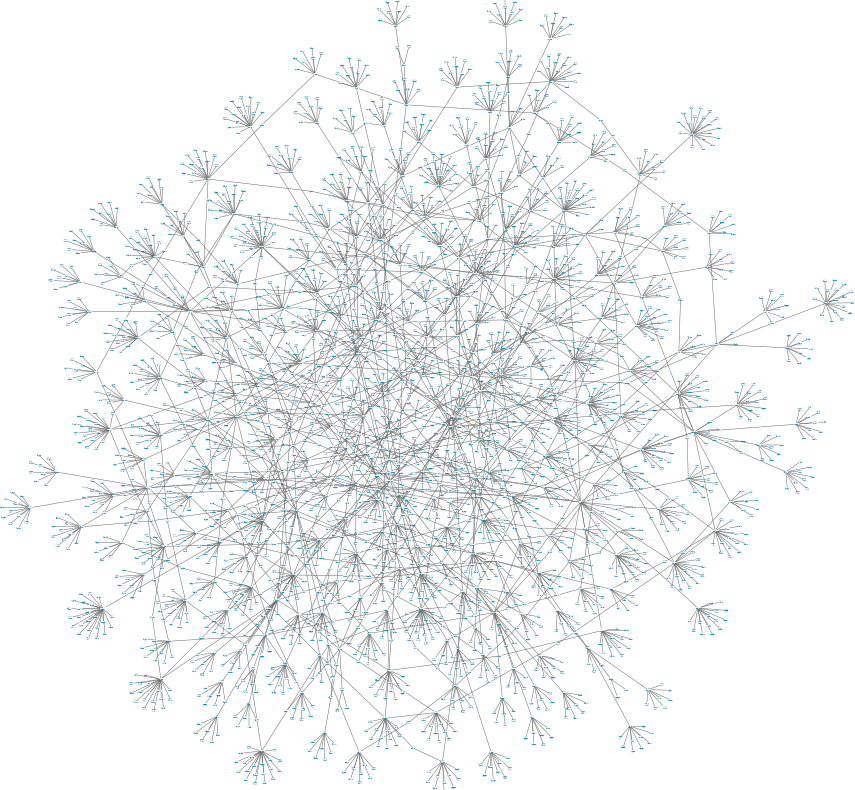
\includegraphics[width=0.4\textwidth]{pics/GraphOfTwitterSpammers}
\caption{Пример взаимосвязей спамовых аккаунтов Twitter}
\label{pic:GraphOfTwitterSpammers}
\end{figure}
Тем не менее, алгоритм CIA позиционируется не как полноценный алгоритм детектирования, а как «легковесный алгоритм вывода и ранжирования», который может быть встроен в систему обнаружения спамеров в комбинации с другими методами \cite{Chao}.

В своей работе Жань \cite{Zhang} предлагает находить потенциальных спамеров как пользователей, имеющих достаточно большое количество твитов, являющимися дубликатами сообщений других пользователей.
Для выявления дублированных твитов среди набора твитов всех пользователей в наборе данных используется метод locality-sensitive hashing (LSH),
 позволяющий оценить коэффициент схожести Жаккара для n-грамм над словами в статусах. Твиты, для которых коэффициент Жаккара превышает 0.8,
 считаются дубликатами. Использование данного метода в детектировании спамеров предполагает дальнейшую классификацию на основе свойств сообщений и профилей,
 характерных для спамеров, имеющих дублированные сообщения.

\end{subsection}

\end{section}
